\documentclass[10pt,a4paper,twocolumn]{article}

\usepackage[T1]{fontenc}
\usepackage[utf8]{inputenc}
\usepackage{amsmath,amssymb,mathtools}
\usepackage{booktabs,tabularx,array,multirow}
\usepackage{graphicx}
\usepackage{xcolor}
\usepackage{geometry}
\usepackage[expansion=false]{microtype}
\usepackage{enumitem}
\usepackage{listings}
\usepackage{fancyhdr}
\usepackage{caption}
\usepackage{tikz}
\usetikzlibrary{arrows.meta,positioning,shapes.geometric,fit,backgrounds,calc}
\usepackage[hidelinks]{hyperref}

\geometry{top=18mm,bottom=20mm,left=17mm,right=17mm,columnsep=7mm,headheight=13pt}
\setlength{\parindent}{1em}
\setlength{\parskip}{0pt}
\setlength{\emergencystretch}{1.5em}
\setlist{nosep,leftmargin=*}
\renewcommand{\arraystretch}{1.12}

\definecolor{salusblue}{HTML}{174A7E}
\definecolor{saluscyan}{HTML}{2B8CBE}
\definecolor{salusgreen}{HTML}{238B45}
\definecolor{salusorange}{HTML}{D95F0E}
\definecolor{saluspurple}{HTML}{756BB1}
\definecolor{salusgray}{HTML}{5D6D7E}
\definecolor{saluslight}{HTML}{EAF2F8}
\definecolor{papergray}{HTML}{F6F7F8}
\hypersetup{colorlinks=true,linkcolor=salusblue,citecolor=salusgreen,urlcolor=salusblue}

\pagestyle{fancy}
\fancyhf{}
\fancyhead[L]{SALUS Entity--Graph Framework}
\fancyhead[R]{UC4 Demonstrator}
\fancyfoot[C]{\thepage}

\lstset{
  basicstyle=\ttfamily\scriptsize,
  backgroundcolor=\color{papergray},
  frame=single,
  rulecolor=\color{gray!35},
  breaklines=true,
  columns=fullflexible,
  showstringspaces=false,
  xleftmargin=1mm,
  xrightmargin=1mm
}

\tikzset{
  layer/.style={draw=salusblue,rounded corners=2pt,thick,fill=saluslight,minimum height=8mm,align=center,font=\small},
  box/.style={draw=salusgray,rounded corners=2pt,fill=white,align=center,font=\scriptsize,inner sep=4pt},
  entity/.style={draw=salusblue,thick,rounded corners,fill=saluslight,align=center,font=\scriptsize,minimum width=17mm,minimum height=8mm},
  process/.style={draw=salusgreen,thick,rounded corners,fill=green!8,align=center,font=\scriptsize,minimum width=17mm,minimum height=8mm},
  policy/.style={draw=salusorange,thick,diamond,aspect=1.8,fill=orange!8,align=center,font=\scriptsize,inner sep=1.5pt},
  data/.style={draw=saluspurple,thick,ellipse,fill=purple!7,align=center,font=\scriptsize,minimum width=17mm,minimum height=8mm},
  arrow/.style={-{Latex[length=2mm]},thick,draw=salusgray},
  evidencearrow/.style={-{Latex[length=2mm]},very thick,draw=saluspurple},
  denyarrow/.style={-{Latex[length=2mm]},thick,dashed,draw=salusorange}
}

\newcommand{\Framework}{\mathcal{F}_{\mathrm{SALUS}}}
\newcommand{\code}[1]{\texttt{#1}}
\newcommand{\R}{\mathbb{R}}
\newcommand{\N}{\mathbb{N}}
\newcommand{\indicator}{\mathbb{I}}

\title{\vspace{-10mm}\textbf{A Source-Traceable Entity--Graph and Hybrid Simulation Framework for SALUS Cyber-Physical Use Cases}\\[1mm]
\large Mathematical Formulation and an Evidence-Governed UC4 Demonstrator}
\author{SALUS mathematical simulation Technical Framework Paper}
\date{8 September 2026}

\begin{document}
\maketitle

\begin{abstract}
Cyber-physical use cases combine heterogeneous physical assets, digital replicas, services, human roles, processes, uncertain observations and policy-governed data exchanges. Describing these dimensions independently creates semantic drift: process diagrams use names not found in data schemas, simulations omit authorization, and analytical claims lose their evidence provenance. This paper introduces a source-traceable entity--graph and hybrid simulation framework developed for the SALUS project. The framework defines a canonical typed entity universe, temporal multigraph relations, BPMN-aligned process semantics, hybrid state and event dynamics, stochastic observation channels, fail-closed authorization, content-addressed evidence, custody chains, evidence-bounded reconstruction and reproducible evaluation.

SALUS Use Case 4 (UC4), a lawful investigation of unauthorized smart-home entry and IoT sensor tampering, is used as the executable demonstrator. Its instantiation contains 38 entities, 123 static relations, seven BPMN models, nine JSON Schemas, a deterministic simulator, 16 negative/edge experiments, a 100-run Monte Carlo design and seven integration contracts. The nominal run preserves 17 verified evidence items with zero bytes released on denied decisions and achieves reconstruction recall 1.0 against isolated synthetic truth. Across the uncertainty design, mean capture recall is 0.8990 and mean reconstruction recall is 0.6647. Forty-seven automated tests validate schemas, graph integrity, process structure, conservation, authorization, custody, truth isolation and reproducibility. The contribution is a reusable engineering method, not evidence of real-pilot performance: synthetic assumptions and external integration boundaries remain explicit and replaceable.
\end{abstract}

\textbf{Keywords---}Cyber-physical systems; Digital Twin; typed property graph; hybrid systems; BPMN; digital evidence; provenance; lawful acquisition; reproducible simulation.

\section{Introduction}

The SALUS project addresses security and resilience across infrastructures that combine physical entities, networks, software services, digital counterparts and human decision makers. the modelling task requires these elements and their processes, information exchanges and relations to be formally and mathematically modelled~\cite{salusproposal}. A practical difficulty is that each modelling view is usually developed in isolation. Entity inventories become spreadsheets, processes become diagrams, simulation variables become code-local names, and evidence handling becomes a narrative control. The resulting artefacts may be individually useful yet impossible to validate as one coherent system.

This paper introduces \(\Framework\), a framework that treats semantic alignment as a first-class system property. A stable entity identifier must retain the same meaning in the source register, JSON instance, relation graph, BPMN process, simulator, runtime graph, evidence record and validation report. A process transition is not merely a drawing: it maps to executable guards and effects. An analytical result is not merely a score: it cites evidence that cites a source record, authorization, policy decision and custody history.

UC4 is used to demonstrate the framework. It concerns a smart-home incident in which a door is opened, a Home Assistant automation responds, and a door sensor is tampered with and disconnected. A distinct case trigger and authorization precede a scoped remote acquisition through CPE and LEA services. This use case stresses the framework because physical truth, network/application observations, Digital Twin state, lawful collectability and investigative inference can diverge.

The framework makes the following contributions:

\begin{enumerate}
  \item a formal canonical entity tuple and typed temporal multigraph that span physical, digital, organizational and evidentiary layers;
  \item an explicit mapping from BPMN process families to a hybrid discrete-event transition system;
  \item a compositional model for observation uncertainty, queue dynamics, Digital Twin synchronization and evidence reconstruction;
  \item an executable authorization predicate in which case creation, authentication, alerts and threat context cannot substitute for lawful scope;
  \item a cryptographically linked evidence/provenance abstraction that supports testable integrity and custody failure paths;
  \item an evaluation protocol that isolates hidden synthetic truth, preserves undefined metrics and records complete seed sets; and
  \item a versioned integration and replacement pattern for extending one demonstrated use case to other SALUS cases and pilot adapters.
\end{enumerate}

\section{Design Requirements}

The SALUS proposal and mathematical simulation roadmap~\cite{salusproposal,frameworkroadmap} imply six framework-level requirements.

\textbf{R1: semantic identity.} Every entity, relationship, event, policy decision, evidence item and custody action requires a stable unique identifier and controlled type.

\textbf{R2: separation of epistemic layers.} Physical state, Digital Twin state, raw/normalized observation, retained source record, collected evidence and analyst conclusion must remain distinct.

\textbf{R3: executable process semantics.} Normal operation, incidents, detection, acquisition and investigation must be represented both as process models and executable transitions.

\textbf{R4: governed information exchange.} Authorization must default to deny and data must be minimized before release and hashing.

\textbf{R5: explicit uncertainty.} Loss, delay, error, clock offset, congestion, retention and missing evidence must be configurable and measurable.

\textbf{R6: reproducible assurance.} Schemas, invariants, negative paths, fixed seeds, confidence intervals, requirements traceability and artifact hashes must support independent review.

Figure~\ref{fig:framework} summarizes the layered framework.

\begin{figure*}[t]
\centering
\resizebox{0.94\textwidth}{!}{%
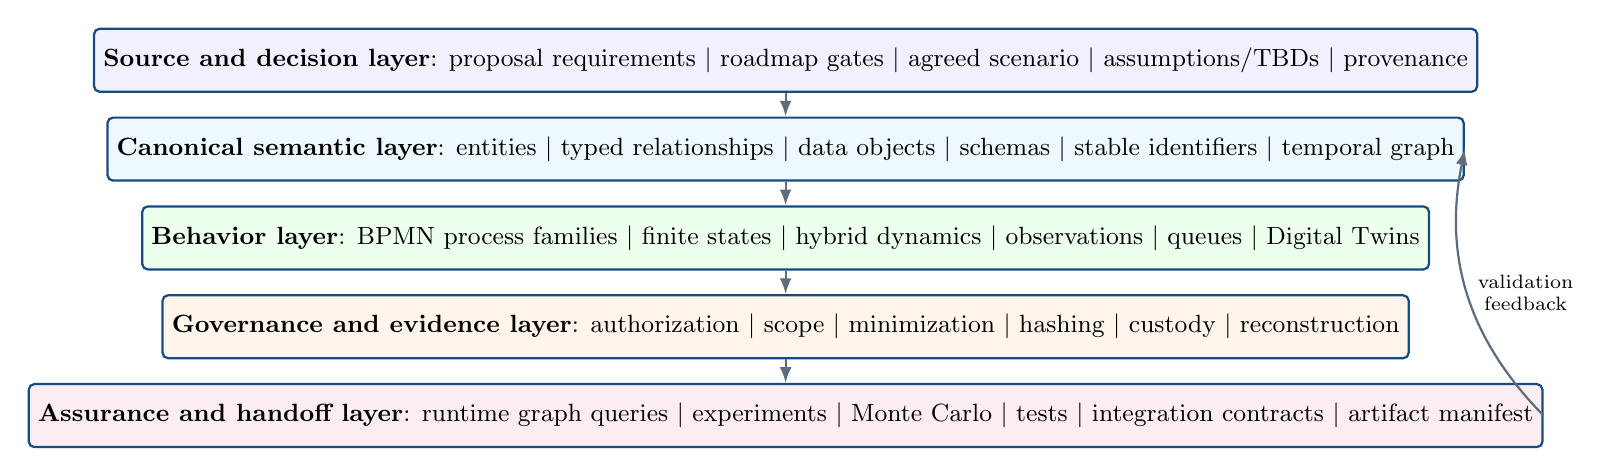
\begin{tikzpicture}[node distance=3mm and 4mm]
  \node[layer,minimum width=0.96\textwidth,fill=blue!6] (sources) {\textbf{Source and decision layer}: proposal requirements $\mid$ roadmap gates $\mid$ agreed scenario $\mid$ assumptions/TBDs $\mid$ provenance};
  \node[layer,below=of sources,minimum width=0.96\textwidth,fill=cyan!7] (semantic) {\textbf{Canonical semantic layer}: entities $\mid$ typed relationships $\mid$ data objects $\mid$ schemas $\mid$ stable identifiers $\mid$ temporal graph};
  \node[layer,below=of semantic,minimum width=0.96\textwidth,fill=green!7] (behavior) {\textbf{Behavior layer}: BPMN process families $\mid$ finite states $\mid$ hybrid dynamics $\mid$ observations $\mid$ queues $\mid$ Digital Twins};
  \node[layer,below=of behavior,minimum width=0.96\textwidth,fill=orange!8] (governance) {\textbf{Governance and evidence layer}: authorization $\mid$ scope $\mid$ minimization $\mid$ hashing $\mid$ custody $\mid$ reconstruction};
  \node[layer,below=of governance,minimum width=0.96\textwidth,fill=purple!7] (assurance) {\textbf{Assurance and handoff layer}: runtime graph queries $\mid$ experiments $\mid$ Monte Carlo $\mid$ tests $\mid$ integration contracts $\mid$ artifact manifest};
  \draw[arrow] (sources) -- (semantic);
  \draw[arrow] (semantic) -- (behavior);
  \draw[arrow] (behavior) -- (governance);
  \draw[arrow] (governance) -- (assurance);
  \draw[arrow,bend left=28] (assurance.east) to node[right,font=\scriptsize,align=center]{validation\\feedback} (semantic.east);
\end{tikzpicture}
}
\caption{The SALUS entity--graph framework. Each layer is machine-readable or executable, and validation links lower-layer results back to canonical semantics and assumptions.}
\label{fig:framework}
\end{figure*}

\section{Canonical Entity--Graph Model}

\subsection{Entity definition}

Let the canonical entity universe be \(\mathcal{V}=\{v_1,\ldots,v_n\}\). An entity is the tuple

\begin{equation}
v_i=\langle id_i,c_i,d_i,o_i,\ell_i,z_i,\Sigma_i,I_i,D_i,P_i\rangle,
\label{eq:entity}
\end{equation}

where \(id_i\) is stable identity, \(c_i\) is entity class, \(d_i\in\{\text{physical},\text{digital},\text{logical}\}\) is designation, \(o_i\) is owner/operator, \(\ell_i\) is location, \(z_i\subseteq\mathcal{Z}\) is zone membership, \(\Sigma_i\) is lifecycle/state vocabulary, \(I_i\) is the interface set, \(D_i\) is generated/consumed data, and \(P_i\) is provenance and sensitivity metadata.

The class function \(c:\mathcal{V}\rightarrow\mathcal{C}\) admits actors, physical environments, devices, gateways, sensors, actuators, services, Digital Twins, zones and data/policy/evidence objects. This is intentionally broader than a network inventory. It gives authorization objects and analytical claims the same traceable identity discipline as physical devices.

\subsection{Typed temporal multigraph}

The static system graph is

\begin{equation}
G_s=(\mathcal{V},\mathcal{E},\tau,\alpha,\nu),
\label{eq:graph}
\end{equation}

where each edge \(e=(u,v,k)\in\mathcal{E}\) has a unique key \(k\), type \(\tau(e)\in\mathcal{T}\), attributes \(\alpha(e)\), and optional validity interval \(\nu(e)=[t_e^-,t_e^+)\). Parallel edges are allowed because two entities may communicate, exchange data and be governed by different policies simultaneously.

The runtime graph adds event, source-record, decision, evidence, custody and claim nodes:

\begin{equation}
G_r(t)=G_s\oplus G_{obs}(t)\oplus G_{pol}(t)\oplus G_{evd}(t)\oplus G_{ana}(t).
\label{eq:runtimegraph}
\end{equation}

The operator \(\oplus\) is a provenance-preserving graph extension, not a graph union that merges nodes by label. Runtime node IDs are globally unique within a run, and all edges resolve to an existing static or runtime node.

\subsection{Physical--digital correspondence}

For physical/device set \(\mathcal{P}\) and twin set \(\mathcal{D}\), the mapping

\begin{equation}
\mu:\mathcal{P}\rightharpoonup\mathcal{D}
\end{equation}

is partial at framework level and bijective over the configured twinned subset:

\begin{equation}
\forall p_1,p_2\in\operatorname{dom}(\mu),\quad \mu(p_1)=\mu(p_2)\Rightarrow p_1=p_2.
\label{eq:twinunique}
\end{equation}

The invariant is represented three ways: physical \code{twin\_id}, twin \code{physical\_entity\_id}, and a \code{MIRRORED\_BY} edge. A synchronization service adds \code{SYNCHRONIZES\_WITH} edges. Validation requires agreement among all representations.

\begin{figure}[t]
\centering
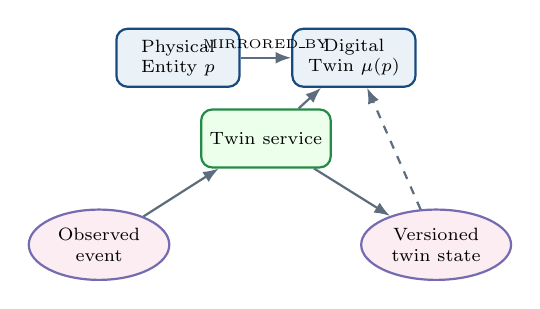
\begin{tikzpicture}[node distance=7mm and 7mm,scale=.92,transform shape]
  \node[entity] (phys) {Physical\\Entity $p$};
  \node[entity,right=of phys] (twin) {Digital\\Twin $\mu(p)$};
  \node[process,below=of $(phys)!0.5!(twin)$] (sync) {Twin service};
  \node[data,below left=of sync] (obs) {Observed\\event};
  \node[data,below right=of sync] (state) {Versioned\\twin state};
  \draw[arrow] (phys) -- node[above,font=\tiny]{MIRRORED\_BY} (twin);
  \draw[arrow] (obs) -- (sync);
  \draw[arrow] (sync) -- (twin);
  \draw[arrow] (sync) -- (state);
  \draw[arrow,dashed] (state) -- (twin);
\end{tikzpicture}
\caption{Canonical physical--digital correspondence. Observation is distinct from both physical truth and accepted twin state.}
\label{fig:twinmapping}
\end{figure}

\subsection{Provenance and assumption status}

Every canonical record carries source references \(S_i\), a record status \(q_i\), confidence \(\gamma_i\), and assumption IDs \(A_i\). An assumption-coverage indicator can be defined as

\begin{equation}
C_{assumed}=\frac{\sum_i\indicator[q_i\in\{\text{assumed},\text{TBD}\}]}{|\mathcal{V}_{en}|+|\mathcal{E}_{en}|}.
\end{equation}

This does not turn provenance into probability. It makes the fraction of model structure resting on replaceable or unknown information visible in every run.

\section{Process and Hybrid-System Semantics}

\subsection{Process families}

The framework partitions a case into five reusable process families: normal operation, incident evolution, detection/case triggering, governed acquisition, and evidence investigation. Each BPMN process \(B_j\) is mapped to a labelled transition system

\begin{equation}
L_j=(S_j,s_j^0,\Lambda_j,\rightarrow_j,F_j),
\end{equation}

where BPMN tasks/events become labels \(\Lambda_j\), exclusive gateways become guarded alternatives, message flows become inter-process exchanges, and end states become \(F_j\). Default branches must be explicit, and non-default exclusive branches require conditions.

\subsection{Hybrid state}

The executable model is

\begin{equation}
\mathcal{M}=\langle\mathcal{Q},X,U,\Delta,F,H,\Omega,\theta\rangle,
\label{eq:hybrid}
\end{equation}

where \(\mathcal{Q}\) is the discrete mode product, \(X\subseteq\R^m\) contains continuous quantities (time, delay, occupancy and lag), \(U\) is configuration/control input, \(\Delta\) is the event-triggered transition relation, \(F\) gives continuous or piecewise updates, \(H\) is the observation mapping, \(\Omega\) contains invariants and guards, and \(\theta\) is the complete parameter/seed vector.

The simulation queue orders events by

\begin{equation}
e_i\prec e_j\iff(t_i<t_j)\lor(t_i=t_j\land s_i<s_j),
\label{eq:ordering}
\end{equation}

where \(s_i\) is a monotonically allocated insertion sequence. Equation~\eqref{eq:ordering} provides deterministic tie breaking across platforms.

\subsection{Observation channel}

For a true event \(x_i(t)\), the observable channel samples delivery

\begin{equation}
d_i\sim\operatorname{Bernoulli}\left((1-p_L)(1-p_{E,i})\right),
\end{equation}

and timestamps a delivered event as

\begin{align}
\hat t_i &=t_i+b_i+\epsilon_i, & |b_i|&\le B_i,\quad |\epsilon_i|\le J,\\
t_i^{ing}&=t_i+\delta_i^{proc}+\delta_i^{net}.&&
\end{align}

The model therefore retains true time (evaluation only), local event time and ingest time as separate concepts. A lost true event cannot update Home Assistant, a Digital Twin or reconstruction.

\subsection{Flow and queue dynamics}

For byte occupancy \(q_k\), arrival \(a_k\), service capacity \(c_k\) and buffer \(K\),

\begin{align}
u_k&=\min(q_k+a_k,c_k),\\
\ell_k&=\max(0,q_k+a_k-u_k-K),\\
q_{k+1}&=q_k+a_k-u_k-\ell_k.
\label{eq:queue}
\end{align}

Consequently,

\begin{equation}
q_k+a_k=u_k+\ell_k+q_{k+1},\qquad 0\le q_{k+1}\le K.
\end{equation}

The executable queue asserts this conservation identity after every update. Background utilization \(\rho_b\) modifies effective service \(c_k=(1-\rho_b)C\Delta t/8\).

\subsection{Digital Twin update}

For accepted twin version \(\bar v_i\), state \(\bar x_i\) and incoming update \((v,x,t_e,t_a)\),

\begin{equation}
(\bar v_i',\bar x_i')=
\begin{cases}
(v,x),&v>\bar v_i,\\
(\bar v_i,\bar x_i),&v\le\bar v_i.
\end{cases}
\end{equation}

Accepted synchronization lag is \(L_i=\max(0,t_a-t_e)\). A stale update increments a rejection counter but does not mutate accepted state. A twin can also become temporally stale if no accepted update arrives before threshold \(L_{max}\).

\section{Governed Evidence Calculus}

\subsection{Authorization predicate}

The release predicate for record \(r\), request \(q\) and evaluation time \(t\) is

\begin{align}
\mathsf{Auth}(r,q,t)={}&D(q)\land V(q)\land P(q)\land T_a(q,t)\land T_e(q,r)\nonumber\\
&\land S_{ent}(q,r)\land S_{data}(q,r)\land S_{act}(q,r),
\label{eq:auth}
\end{align}

where \(D\) is an explicit allow path, \(V\) is authorization verification, \(P\) is exact purpose match, \(T_a\) and \(T_e\) are authorization/evidence windows, and \(S_{ent},S_{data},S_{act}\) are entity, data and action scope. The default is false. Case triggers, login state, AI alerts, threat context and network policy do not occur in Eq.~\eqref{eq:auth} and cannot authorize evidence.

If Eq.~\eqref{eq:auth} is true, field minimization is

\begin{equation}
\pi_F(r)=\{(k,r[k]):k\in F\cap\operatorname{keys}(r)\}.
\end{equation}

The evidence creation function is partial:

\begin{equation}
\mathsf{Collect}(r,q)=
\begin{cases}
\mathsf{Evidence}(\pi_F(r)),&
\begin{aligned}\mathsf{Auth}&=1,\\[-2pt]|\pi_F(r)|&>0,
\end{aligned}\\
\bot,&\text{otherwise}.
\end{cases}
\label{eq:collect}
\end{equation}

The bottom value \(\bot\) emits an auditable deny decision with empty released fields and zero bytes, never an evidence payload.

\subsection{Evidence and custody}

For canonical serialization \(J\), the content identity of evidence \(e\) is

\begin{equation}
h_e=\operatorname{SHA256}(J(e.content)).
\end{equation}

The custody sequence uses genesis \(c_0\) derived from run, case and schema version, then

\begin{equation}
c_k=\operatorname{SHA256}(c_{k-1}\Vert h_e\Vert a_k\Vert t_k\Vert u_k).
\label{eq:custody}
\end{equation}

Verification recomputes every link and sequence number. Failure produces \code{verification\_failed}; the implementation never silently repairs a chain or calls it a production blockchain.

\subsection{Evidence-bounded reconstruction}

Let \(E_v\) be the set of content- and custody-verified evidence. Reconstruction is a function

\begin{equation}
\mathcal{R}:E_v\times\Theta_R\rightarrow(O_R,C_R),
\end{equation}

where \(O_R\) is a normalized observation set and \(C_R\) is a set of qualified claims. Claim support is transparently aggregated:

\begin{equation}
s(c)=\operatorname{clip}_{[0,1]}\left(
\frac{\sum_{e\in E_c}w_{type(e)}\gamma_{source(e)}}{\sum_{e\in E_c}w_{type(e)}}
-\lambda m_c\right),
\label{eq:support}
\end{equation}

where \(E_c\subseteq E_v\), \(w\) are declared type weights, \(\gamma\) is source reliability, \(m_c\) measures missing expected observations and \(\lambda\) is a penalty. Each claim retains evidence IDs, an uncertainty interval, missing observations and alternative explanations.

\begin{figure*}[t]
\centering
\resizebox{0.94\textwidth}{!}{%
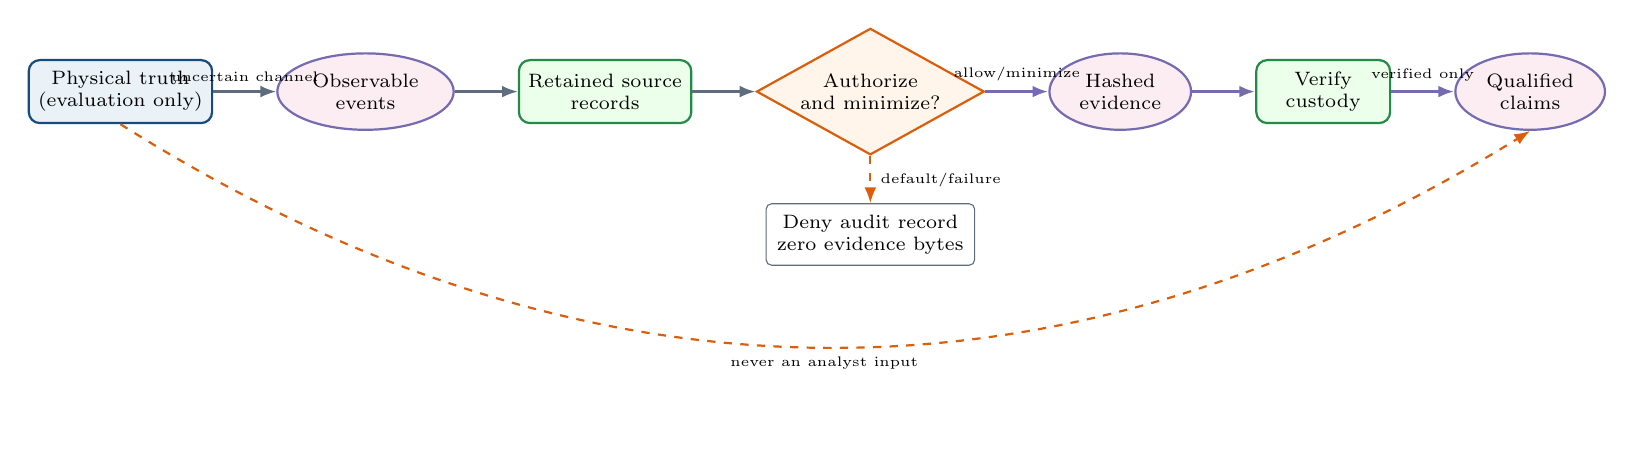
\begin{tikzpicture}[node distance=8mm and 8mm]
  \node[entity] (truth) {Physical truth\\(evaluation only)};
  \node[data,right=of truth] (obs) {Observable\\events};
  \node[process,right=of obs] (retain) {Retained source\\records};
  \node[policy,right=of retain] (auth) {Authorize\\and minimize?};
  \node[data,right=of auth] (evidence) {Hashed\\evidence};
  \node[process,right=of evidence] (custody) {Verify\\custody};
  \node[data,right=of custody] (claims) {Qualified\\claims};
  \draw[arrow] (truth) -- node[above,font=\tiny]{uncertain channel} (obs);
  \draw[arrow] (obs) -- (retain);
  \draw[arrow] (retain) -- (auth);
  \draw[evidencearrow] (auth) -- node[above,font=\tiny]{allow/minimize} (evidence);
  \draw[evidencearrow] (evidence) -- (custody);
  \draw[evidencearrow] (custody) -- node[above,font=\tiny]{verified only} (claims);
  \node[box,below=6mm of auth] (deny) {Deny audit record\\zero evidence bytes};
  \draw[denyarrow] (auth) -- node[right,font=\tiny]{default/failure} (deny);
  \draw[denyarrow,bend right=32] (truth.south) to node[below,font=\tiny]{never an analyst input} (claims.south);
\end{tikzpicture}
}
\caption{Evidence-governed information path. Hidden truth can score the final reconstruction but cannot enter collection, evidence or claim construction.}
\label{fig:evidencepipeline}
\end{figure*}

\section{Framework Invariants and Execution Algorithm}

The framework defines the following testable invariants:

\begin{align}
\textbf{I1:}&\quad id_i=id_j\Rightarrow i=j \quad\text{within each identifier domain},\\
\textbf{I2:}&\quad \operatorname{ends}(e)\subseteq\mathcal{V},\\
\textbf{I3:}&\quad 0\le q_k\le K\quad\land\quad\text{queue conservation},\\
\textbf{I4:}&\quad \mathsf{deny}\Rightarrow bytes_{released}=0\land E_{new}=\emptyset,\\
\textbf{I5:}&\quad c\in C_R\Rightarrow evidenceIDs(c)\subseteq IDs(E_v),\\
\textbf{I6:}&\quad V_{truth}\cap V(G_r)=\emptyset,\\
\textbf{I7:}&\quad seed_1=seed_2\land config_1=config_2\\
&\quad\Rightarrow hash_1=hash_2.
\end{align}

The end-to-end procedure is shown below.

\begin{lstlisting}[language={},caption={Framework execution procedure.}]
INPUT: versioned config C, canonical entities V,
       relationships E, BPMN/process contracts B, seed z
1 validate schemas, versions, IDs, references, graph,
  process structure, cross-field bounds and integrations
2 instantiate physical, application, queue and twin states
3 schedule initial events using (time, insertion_sequence)
4 while event queue is non-empty and time <= horizon:
      apply legal transition and physical constraints
      emit hidden truth where the simulator owns truth
      sample observable channel from injected seed streams
      retain observable records and update graph/twins
      if acquisition event:
          evaluate authorization per record
          minimize eligible content before hashing
          append and verify custody; quarantine failures
          reconstruct from verified evidence only
5 evaluate reconstruction against isolated truth
6 compute explicit metrics; preserve undefined denominators
7 canonically serialize outputs and compute result hash
8 run declared branches/seed design; emit validation evidence
OUTPUT: validated run package, graph, metrics and hashes
\end{lstlisting}

\section{UC4 Demonstrator}

\subsection{Instantiation}

UC4 instantiates \(\Framework\) with a smart-home environment, three network zones, six physical/device entities and six Digital Twins. The devices are an open-source CPE router, Home Assistant host, door/window contact sensor, presence sensor, smart plug and smart light. Services represent optional cloud, lawful interception, evidence storage, custody, reconstruction and Digital Twin operations. Human/system roles represent the resident, investigator, authorizing authority, CPE/operator support, unauthorized actor and auditor.

The canonical UC4 graph has 38 entities and 123 typed relations, including 37 membership-to-use-case, 13 zone membership, ten generation, six deployment, six ownership, six mirror, six synchronization, and further routing, communication, observation, collection, evidence, authorization, custody, protection, trigger and correlation edges.

\subsection{Scenario timeline}

Figure~\ref{fig:uc4timeline} maps the demonstrator to the generic process families.

\begin{figure*}[t]
\centering
\resizebox{0.94\textwidth}{!}{%
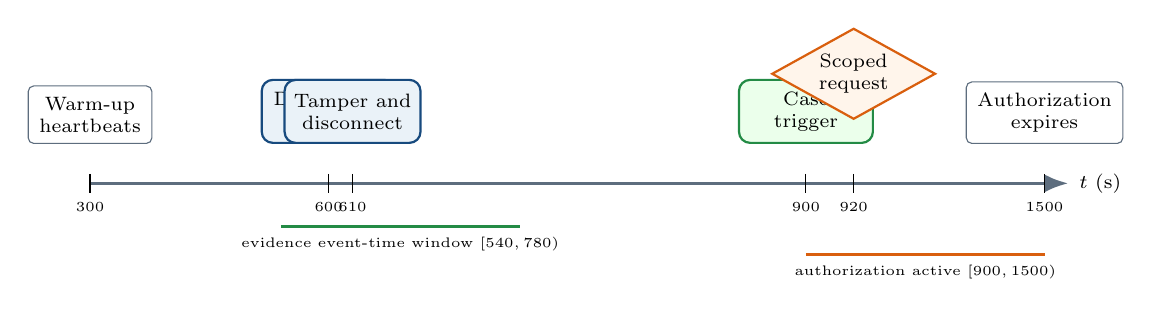
\begin{tikzpicture}[x=0.0125\textwidth,y=1cm]
  \draw[very thick,draw=salusgray,-{Latex}] (0,0) -- (82,0) node[right,font=\scriptsize] {$t$ (s)};
  \foreach \x/\lab in {0/300,20/600,22/610,60/900,64/920,80/1500}{
    \draw (\x,0.12) -- (\x,-0.12) node[below,font=\tiny] {\lab};
  }
  \node[box,above=5mm] at (0,0) {Warm-up\\heartbeats};
  \node[entity,above=5mm] at (20,0) {Door opens\\presence};
  \node[entity,above=5mm] at (22,0) {Tamper and\\disconnect};
  \node[process,above=5mm] at (60,0) {Case\\trigger};
  \node[policy,above=8mm] at (64,0) {Scoped\\request};
  \node[box,above=5mm] at (80,0) {Authorization\\expires};
  \draw[very thick,draw=salusgreen] (16,-0.55) -- (36,-0.55) node[midway,below,font=\tiny]{evidence event-time window $[540,780)$};
  \draw[very thick,draw=salusorange] (60,-0.9) -- (80,-0.9) node[midway,below,font=\tiny]{authorization active $[900,1500)$};
\end{tikzpicture}
}
\caption{UC4 scenario timing. The evidence event-time window and authorization activity window are distinct constraints.}
\label{fig:uc4timeline}
\end{figure*}

At \(t=600\)~s an unauthorized actor opens the entrance. The door and presence sensors may report the event; Home Assistant can trigger a light. At \(t=610\)~s the door sensor is tampered with and becomes offline. A case trigger occurs at \(t=900\)~s and a collection request at \(t=920\)~s. The incident is inside the evidence window \([540,780)\), while authorization is active over \([900,1500)\). Record event time determines evidentiary scope; acquisition time determines authorization activity.

\subsection{Process and graph realization}

Seven BPMN~2.0 files represent the five process families, system collaboration and critical lifecycles. Their pools separate home, CPE and LEA boundaries. The runtime graph adds observed events, policy decisions, evidence, custody and claims to the static graph. In the nominal run it contains 171 nodes and 408 edges, answers nine competency queries, and excludes hidden truth by schema and test.

\section{Evaluation Method}

\subsection{Metrics}

Evidence capture recall and precision are

\begin{align}
R_E&=\frac{|E_{relevant,preserved}|}{|R_{relevant,observable}|},\\
P_E&=\frac{|E_{relevant,preserved}|}{|E_{preserved}|}.
\end{align}

Reconstruction recall/precision match relevant reconstructed events \(M\) against isolated relevant truth \(T\):

\begin{align}
R_R&=\frac{|M|}{|T|}, & P_R&=\frac{|M|}{|O_R|},\\
MAE_t&=\frac{1}{|M|}\sum_{(i,j)\in M}|\hat t_i-t_j|.&&
\end{align}

Undefined denominators produce \code{null}, never zero. Other metrics include unauthorized disclosure count/bytes, latency, loss by source/cause, custody failure, twin lag/staleness, queue occupancy/loss/utilization and assumption coverage.

\subsection{Experiments}

The evaluation contains: (i) a deterministic nominal case; (ii) 15 additional branches for authorization, observation, retention, congestion, timing, corruption and service availability; and (iii) 100 Monte Carlo runs. The Monte Carlo design samples observation loss \([0,0.30]\), clock bound \([0,30]\)~s, background load \([0,0.95]\), sensor error \([0,0.25]\), and collection delay \([0,650]\)~s. Master seed 20260908 generates samples; simulation seeds 44000--44099 are recorded.

Continuous means use two-sided 95\% normal-approximation intervals with sample standard deviation; binary proportions use Wilson intervals. Pearson \(r\) is reported as descriptive sensitivity only.

\section{Results}

\subsection{Nominal and uncertainty outcomes}

\begin{table}[t]
\centering
\caption{UC4 nominal and Monte Carlo outcomes.}
\label{tab:results}
\resizebox{\columnwidth}{!}{%
\begin{tabular}{@{}lrr@{}}
\toprule
Metric & Nominal & MC mean [95\% CI] \\
\midrule
Capture recall & 1.000 & 0.899 [0.839, 0.959] \\
Evidence precision & 1.000 & 1.000 [1.000, 1.000] \\
Evidence items & 17 & 10.78 [9.70, 11.86] \\
Recon. recall & 1.000 & 0.665 [0.605, 0.725] \\
Recon. precision & 0.500 & 0.500 [0.500, 0.500] \\
Timestamp MAE (s) & 0.042 & 0.039 [0.035, 0.043] \\
Twin lag (s) & 0.488 & 4.872 [4.235, 5.509] \\
Investigation (s) & 20.017 & 327.70 [289.31, 366.09] \\
Disclosure bytes & 0 & 0.000 [0.000, 0.000] \\
Custody failures & 0 & 0.000 [0.000, 0.000] \\
\bottomrule
\end{tabular}
}
\end{table}

The nominal run preserves and verifies 17 evidence items, generates three strong claims, and releases zero unauthorized bytes. Reconstruction recall is 1.0. Precision is 0.5 because multiple source-specific records preserve corroboration and normalize to relevant event observations, whereas evaluation matches one-to-one against five truth events. This exposes, rather than hides, the future need for calibrated multi-source event fusion.

In the Monte Carlo study, 11 runs preserve no evidence. Their precision and evidence-dependent timing/error metrics are undefined and excluded from corresponding means. The Wilson lower bound for observing zero unauthorized disclosure in 100 tested paths is approximately 0.963; this describes tested software paths, not legal compliance.

\subsection{Negative paths}

All 16 branch-specific assertion sets pass. Absent, invalid, expired, revoked and out-of-scope authorization produce no evidence. Forced door loss removes its downstream Home Assistant automation support. Retention eviction produces an explicit empty-window denial. CPE overflow yields a queue-loss rate of 0.8687 while non-CPE sources survive. Evidence content tampering quarantines one item; tampering with the first custody link makes every downstream item unverified.

\subsection{Sensitivity}

Figure~\ref{fig:sensitivity} visualizes the largest absolute pairwise correlations.

\begin{figure}[t]
\centering
\resizebox{0.97\columnwidth}{!}{%
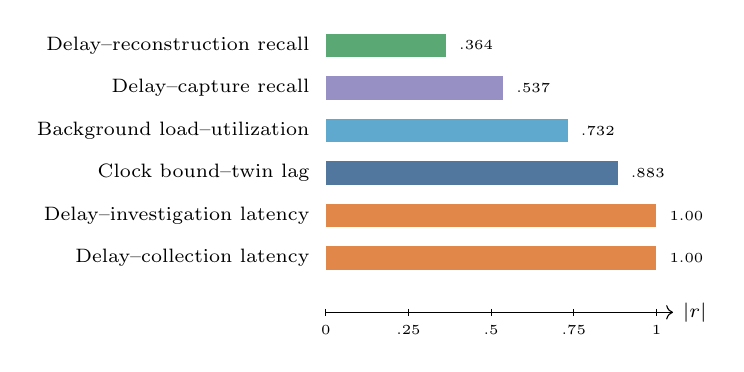
\begin{tikzpicture}[x=4.2cm,y=0.54cm,font=\scriptsize]
  \draw[->] (0,0) -- (1.05,0) node[right] {$|r|$};
  \foreach \x in {0,.25,.5,.75,1}{\draw (\x,.08)--(\x,-.08) node[below,font=\tiny]{\x};}
  \foreach \y/\val/\name/\col in {
    1/1.00/Delay--collection latency/salusorange,
    2/1.00/Delay--investigation latency/salusorange,
    3/.883/Clock bound--twin lag/salusblue,
    4/.732/Background load--utilization/saluscyan,
    5/.537/Delay--capture recall/saluspurple,
    6/.364/Delay--reconstruction recall/salusgreen}{
      \fill[\col!75] (0,\y) rectangle (\val,\y+.55);
      \node[anchor=east] at (-.02,\y+.275) {\name};
      \node[anchor=west,font=\tiny] at (\val+.01,\y+.275) {\val};
  }
\end{tikzpicture}
}
\caption{Largest absolute Pearson sensitivities in the declared synthetic design. Direction is negative for the two delay--recall relations and positive otherwise. Correlation is descriptive, not causal.}
\label{fig:sensitivity}
\end{figure}

Collection delay dominates collection and investigation latency by construction and can reduce capture once retention or authorization boundaries are crossed. Clock uncertainty affects apparent twin lag, and background traffic affects effective acquisition utilization. These mechanistically consistent results demonstrate framework traceability from a parameter to state dynamics and system metrics.

\section{Validation and Reproducibility}

The repository has nine Draft 2020-12 schemas, 38 entities, 123 relationships, seven BPMN files and seven integration contracts. A clean Python 3.12 environment installed the exact lock, passed \code{pip check}, and executed 47 tests with zero failures, errors or skips.

Validation spans schema/meta-schema conformance, strict runtime round trips, migrations, controlled vocabularies, ID uniqueness, endpoint resolution, graph connectivity, twin bijection, BPMN guarded branches and diagram interchange, physical bounds, time monotonicity, queue conservation, authorization terms, minimization, zero-byte denial, content/custody corruption, truth isolation, equal/different seeds, output completeness, query resolution, confidence intervals and manifest tamper detection.

The generated result hash excludes the wall-clock manifest timestamp. The Monte Carlo ledger retains each input, simulation seed, output, canonical run hash and sample hash, plus an ordered aggregate hash. The final handoff manifest similarly lists file size and SHA-256 for every deliverable but excludes itself to avoid recursive hashing.

\section{Generalization Beyond UC4}

UC4 is one instantiation of \(\Framework\), not the framework definition. A new SALUS use case \(u\) can be represented by the configuration

\begin{equation}
\Phi_u=\langle\mathcal{V}_u,\mathcal{E}_u,\mathcal{B}_u,\mathcal{M}_u,\mathcal{P}_u,\Theta_u,\mathcal{K}_u\rangle,
\end{equation}

where \(\mathcal{V}_u,\mathcal{E}_u\) instantiate the canonical graph, \(\mathcal{B}_u\) contains process families, \(\mathcal{M}_u\) specializes hybrid dynamics, \(\mathcal{P}_u\) defines policy/evidence semantics, \(\Theta_u\) contains explicit assumptions and parameters, and \(\mathcal{K}_u\) contains validation and competency questions.

The reusable core is stable identity, provenance, event timing, graph extension, policy-decision/evidence/custody linking, seeded execution and validation. Use-case-specific elements are the entity classes used, state vocabularies, event generators, process guards, authorization vocabulary, reconstruction logic and calibrated distributions.

To add a case safely:

\begin{enumerate}
  \item freeze a bounded scenario and source precedence;
  \item instantiate canonical entities/relations with assumptions;
  \item define five process families and critical lifecycles;
  \item specialize \(\mathcal{M}\) with units, guards and invariants;
  \item define data release and evidence semantics before simulation;
  \item specify competency questions and adverse branches;
  \item execute deterministic and uncertainty evaluation; and
  \item publish integration/replacement contracts and a hash manifest.
\end{enumerate}

This sequence allows domain variation while retaining a comparable assurance structure across SALUS cases.

\section{Integration Architecture}

Seven versioned contracts bind UC4 to adjacent SALUS tasks: T4.4 Digital Twin state/control, T4.2 SDaaSS zones and flows, T3.3 AI/XAI features and alerts, T3.4 threat context, T3.5 device identification and lawful acquisition, T3.1/T3.6 evidence/custody/sharing, and WP6 pilot replacement. Each declares direction, schema, required fields, semantics, authorization, failure paths, assumptions and replacement procedure.

The contracts deliberately distinguish four applicability states: internally implemented, abstract adapter, disabled by default and pilot replacement. Therefore a valid contract does not imply a deployed endpoint. In particular, SDN is disabled, AI/XAI and threat-intelligence services are abstract, and deployment encryption/RBAC/KMS and evidence sharing require external integration.

\section{Discussion}

\subsection{Contribution of graph--process--evidence alignment}

The central contribution is alignment rather than any single algorithm. Equation~\eqref{eq:entity} supplies stable objects; Eq.~\eqref{eq:graph} links them; BPMN supplies human-readable operational structure; Eq.~\eqref{eq:hybrid} makes behavior executable; Eq.~\eqref{eq:auth} governs release; Eqs.~\eqref{eq:collect} and~\eqref{eq:custody} make evidence traceable; Eq.~\eqref{eq:support} bounds inference; and the runtime graph connects all outputs for querying.

This chain gives negative results semantics. An incident without an observation is distinct from no incident. An observation outside an evidence window is distinct from corrupt evidence. A valid authorization with an out-of-scope record is distinct from invalid authorization. Verified content with a broken custody chain is distinct from missing content. An unsupported claim is retained as an analytical state rather than upgraded or discarded.

\subsection{Privacy and epistemic discipline}

The framework encodes privacy-relevant properties structurally: hidden truth separation, metadata-only CPE capture, inactive-by-default collection, per-record authorization, exact purpose, minimization before hashing, zero-byte denial, provenance-linked evidence and evidence-only claims. These properties are testable but do not replace legal analysis.

Epistemic discipline is equally important. Source status, assumption coverage, missing observations, uncertainty intervals, alternative explanations and undefined denominators prevent the model from appearing more certain than its input. In a Digital Twin setting, this matters because a digital state can be stale, partial or derived rather than a perfect image of physical reality.

\section{Threats to Validity and Limitations}

\textbf{Construct validity.} Transparent weighted reconstruction and one-to-one event matching are engineering abstractions. They do not constitute a validated forensic inference model. Queueing is byte-level, not packet-level.

\textbf{Internal validity.} Deterministic tests and negative branches strongly validate implementation invariants, but unmodelled bugs or interactions can remain. Pearson sensitivity does not capture nonlinear interactions.

\textbf{External validity.} Device behavior, network conditions, retention and clocks are synthetic. No real CPE, Home Assistant, SDN, AI/XAI, threat-intelligence or evidence-sharing endpoint is connected. Candidate datasets have not been calibrated.

\textbf{Legal and operational validity.} Synthetic authorization is not legal authority; a hash chain is not an admissibility ruling; passing tests does not prove GDPR compliance, production security or pilot KPI attainment.

The replacement strategy is to preserve canonical contracts while introducing approved measurements, units, firmware/context provenance and adapters in new versioned configurations, then rerun the same validation and uncertainty gates.

\section{Conclusion}

This paper presented \(\Framework\), a mathematical and executable entity--graph framework for SALUS cyber-physical use cases. It unifies source governance, canonical semantics, typed temporal graphs, BPMN processes, hybrid dynamics, Digital Twin synchronization, authorization, evidence, custody, reconstruction and reproducible assurance. UC4 demonstrates the framework end to end without conflating synthetic truth, observable data, legally collectible evidence and analytical conclusions.

The demonstrator is internally complete: 47 tests pass, adverse branches behave as declared, uncertainty is recorded rather than hidden, and integration boundaries are versioned. The broader contribution is a repeatable route from proposal narrative to an executable and falsifiable case model. Future SALUS cases can reuse the semantic and assurance core while specializing their entities, dynamics, policies, processes and calibrated adapters.

\begin{thebibliography}{9}

\bibitem{salusproposal}
SALUS Consortium,
\emph{SALUS Project Proposal, SEP-211108743},
technical proposal, especially pp.~162--164, 169--171 and 190.

\bibitem{frameworkroadmap}
SALUS mathematical simulation Team,
\emph{SALUS HUA mathematical simulation Roadmap},
project roadmap and phased entity/process modelling guidance.

\bibitem{bpmnstandard}
Object Management Group,
\emph{Business Process Model and Notation (BPMN), Version 2.0.2}, 2014.

\bibitem{jsonschema}
JSON Schema Project,
\emph{JSON Schema Core and Validation, Draft 2020-12}.

\bibitem{uc4model}
SALUS mathematical simulation UC4 Implementation,
\emph{UC4 Formal Hybrid Mathematical Model and Executable Repository}, version 0.1.0, 2026.

\end{thebibliography}

\end{document}
